Trong thiết kế hướng tên miền, Kho lưu trữ (Repository) hoạt động như một tập hợp các đối tượng tổng hợp trong bộ nhớ. Tất cả tương tác với bộ lưu trữ dữ liệu được gói gọn bởi đối tượng kho lưu trữ. Kho lưu trữ là một sự trừu tượng hóa trên lớp lưu giữ lâu dài, cung cấp một cách để lưu trữ và truy xuất các đối tượng miền. Lợi ích chính của việc sử dụng kho lưu trữ là giữ cho mô hình miền độc lập với lớp lưu trữ và dễ dàng kiểm thử.

% trong khi ẩn các chi tiết về cách chúng được lưu giữ lâu dài. Mẫu kho lưu trữ cho phép lớp miền duy trì cơ chế tồn tại bất khả tri và cho phép sử dụng các công nghệ lưu trữ khác nhau mà không ảnh hưởng đến mô hình miền.

% <!--hướng dẫn 7/11-->

% <!--hướng dẫn 7/11-->

% <!--hướng dẫn 7/11-->

\begin{example} Trong lập trình, kho lưu trữ luôn được thực hiện là giao diện (interface) và sau đó sử dụng bộ điều hợp tương tác với Repository trong ORM:

\begin{figure}[H]

\centering

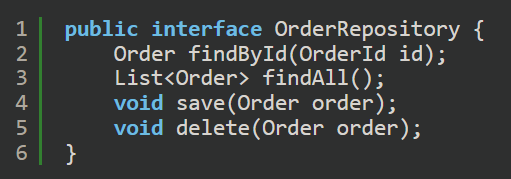
\includegraphics[scale = 0.8]{pictures/_vi_du_lap_trinh_kho_luu_tru_repository/main.png}

\caption{Ví dụ lập trình kho lưu trữ (Repository)}

\end{figure}

\end{example}